\begin{figure}[H]
\centering
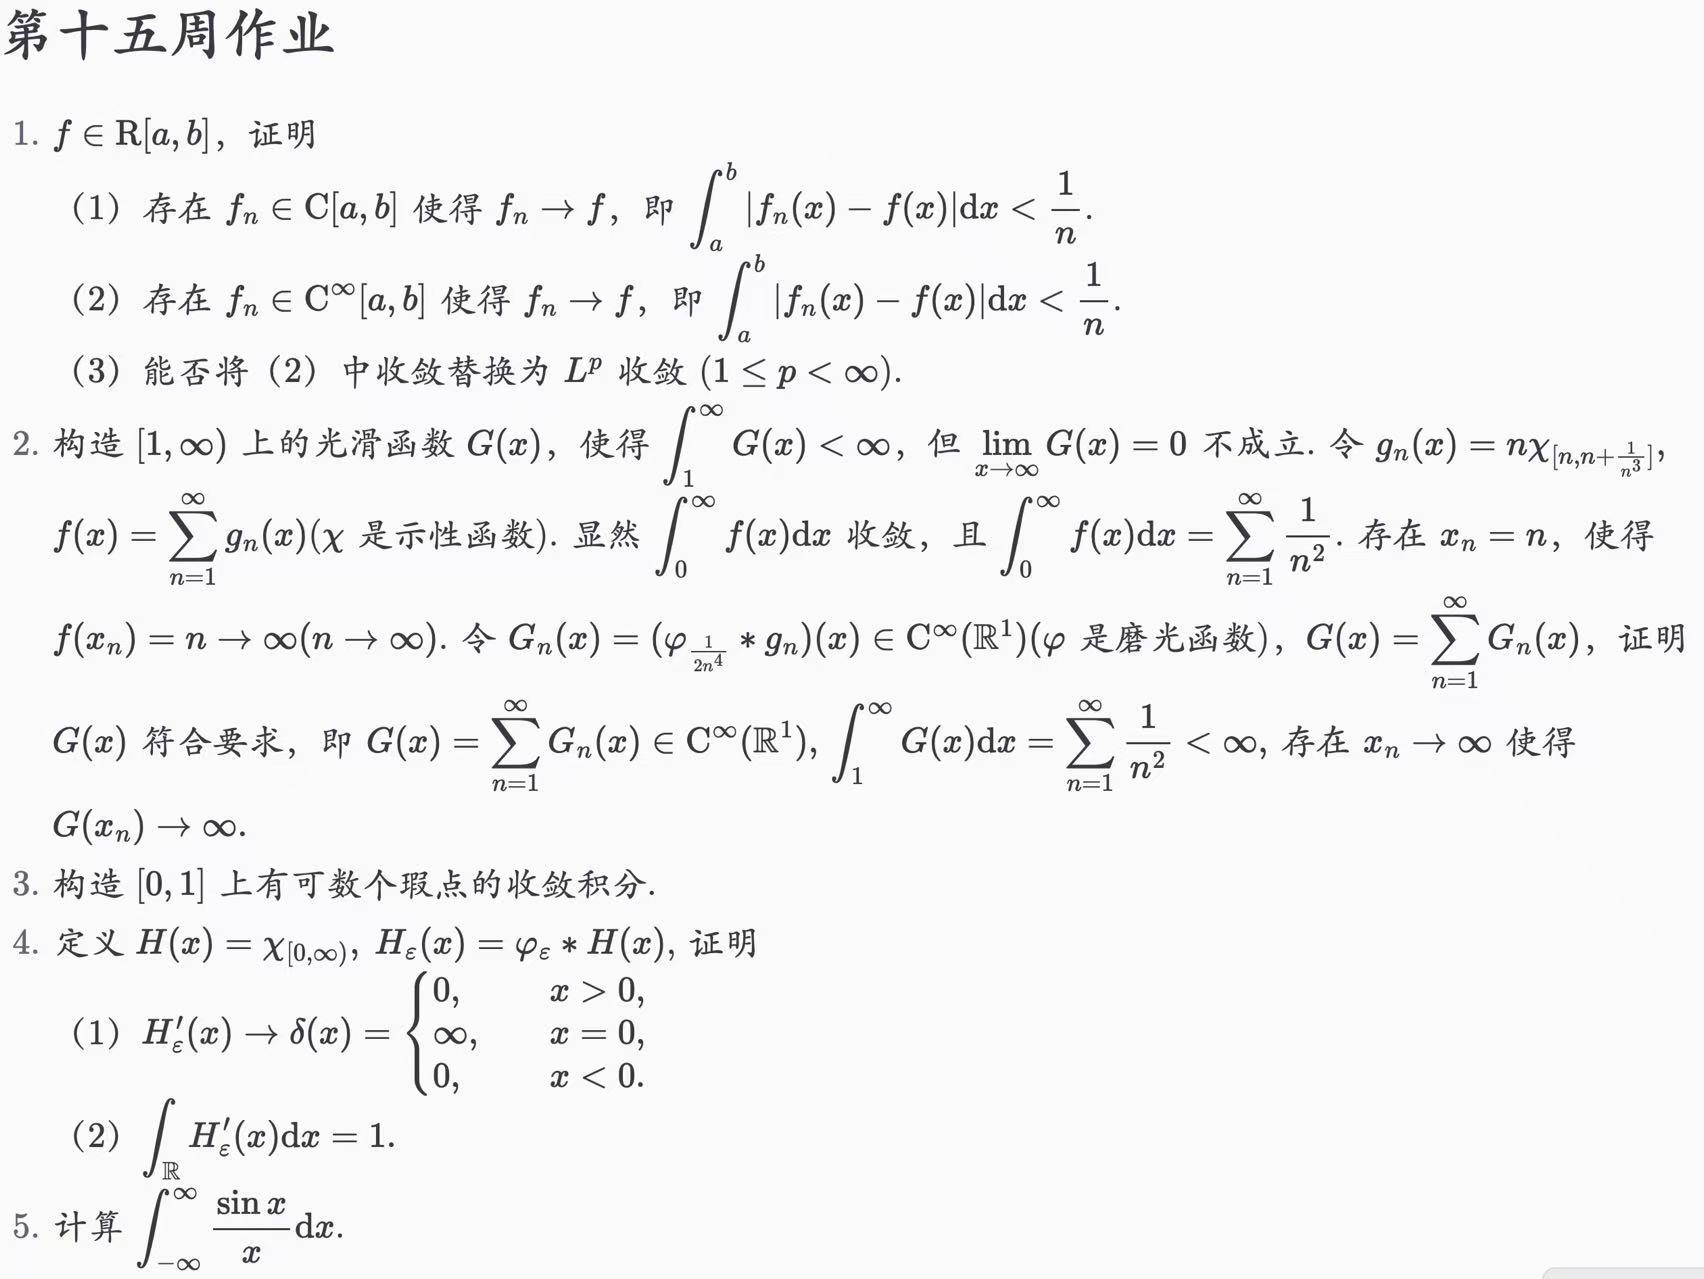
\includegraphics[width=\textwidth]{00b7b55dc72b4229cd5e4979ceae16d3.jpg}
% \caption{}
\label{}
\end{figure}

\begin{exercise}
$f \in \mathrm{R}[a, b]$ ,证明
	\begin{enumerate}
		\item 存在 $f_n \in \mathrm{C}[a, b]$ 使得 $f_n \rightarrow f$ ,即 $\int_a^b\left|f_n(x)-f(x)\right| \mathrm{d} x<\frac{1}{n}$ .
		\item 存在 $f_n \in \mathrm{C}^{\infty}[a, b]$ 使得 $f_n \rightarrow f$ ,即 $\int_a^b\left|f_n(x)-f(x)\right| \mathrm{d} x<\frac{1}{n}$ .
		\item 能否将(2)中收敛替换为 $L^p$ 收敛 $(1 \leq p<\infty)$ .
	\end{enumerate}
\end{exercise}
更强地,我们证明:

\begin{theorem}
设 $u$ 是开集 $\Omega \subseteq \mathbf{R}^n$ 上的有限可积函数.则对 $\Omega$ 的任意有界开子集 $U$ 成立
\[
\lim _{\varepsilon \rightarrow 0} \int_U\left|u_{\varepsilon}(x)-u(x)\right| \mathrm{d} x=0
\]
\end{theorem}
其中 $u_{\varepsilon}(x)\coloneqq (\phi_{\varepsilon}*u)(x)$.

用 $\phi$ 表示 $\mathbf{R}^n$ 上的下列紧支函数:
\[
\phi(x)= \begin{cases}c^{-1} \mathrm{e}^{-\frac{1}{1-|x|^2}}, & |x|<1 \\ 0, & |x| \geqslant 1\end{cases}
\]
其中 $c=\int_{|x|<1} \mathrm{e}^{-\frac{1}{1-|x|^2}} \mathrm{~d} x$ .易知 $\phi \in C^{\infty}\left(\mathbf{R}^n\right)$ 且具有以下性质:
(i)$\phi \geqslant 0$ 且是球对称函数;
(ii) $\operatorname{supp} \phi=\overline{B_1(0)}$ ;
(iii) $\int_{\mathbf{R}^n} \phi(x) \mathrm{d} x=\int_{|x|<1} \phi(x) \mathrm{d} x=1$ .
\[
\phi_{\varepsilon}(x)\coloneqq \frac{1}{\varepsilon^{n}}\phi\left( \frac{x}{\varepsilon} \right)
\]
\begin{proof}
\begin{figure}[H]
\centering
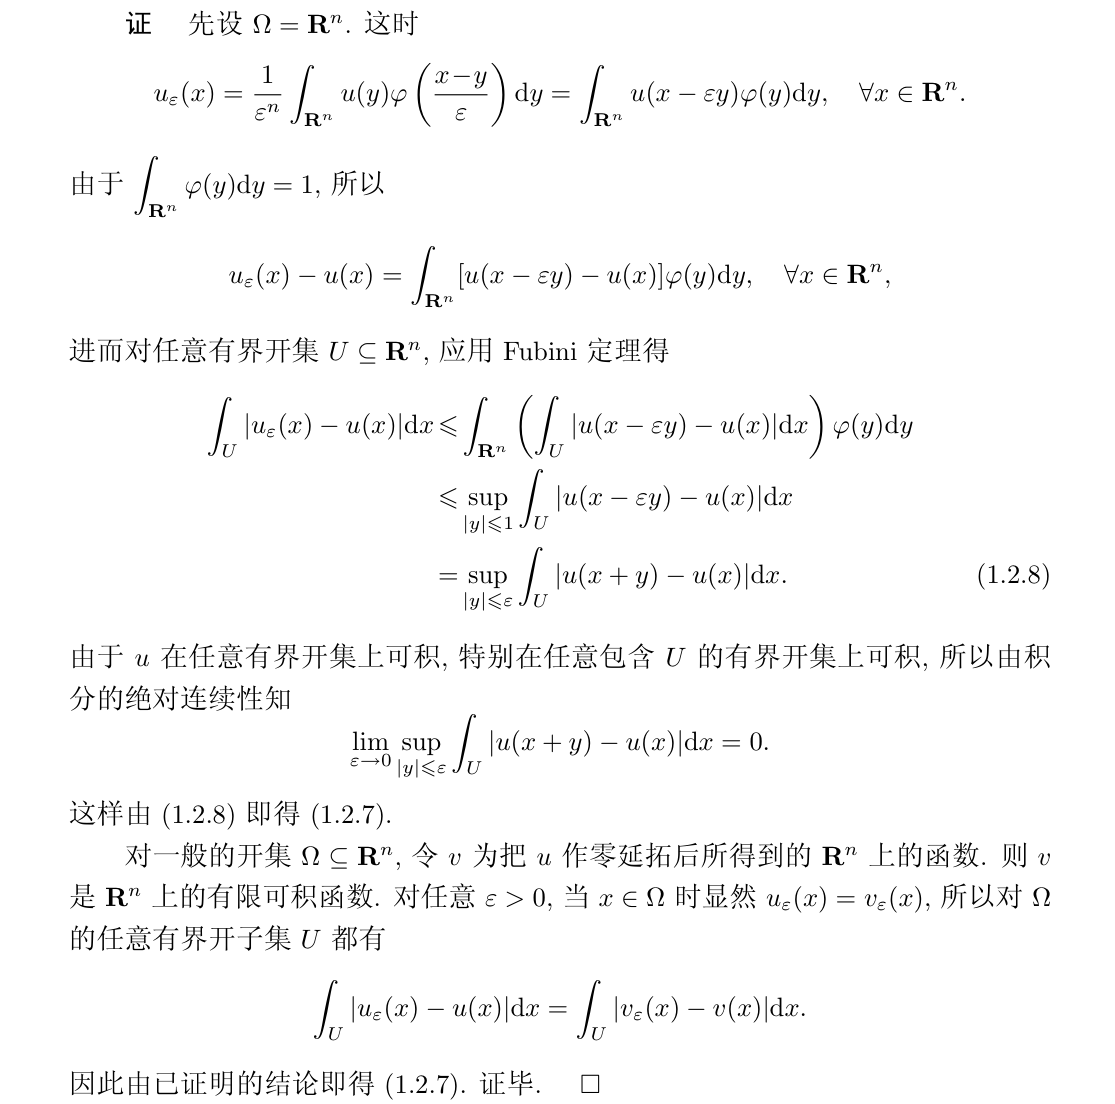
\includegraphics[width=\textwidth]{hw14-2025060800.png}
% \caption{}
\label{}
\end{figure}

\end{proof}
(3) 对于 $L^{p}$ ($1\leq p<\infty$) 收敛也是对的,首先闭区间上的黎曼可积函数(不连续点零测)显然 $L^{p}$ 可积,所以类似地利用积分的绝对连续性即可.

\begin{exercise}
构造 $[1, \infty)$ 上的光滑函数 $G(x)$ ,使得 $\int_1^{\infty} G(x)<\infty$ ,但 $\lim _{x \rightarrow \infty} G(x)=0$ 不成立.令 $g_n(x)=n \chi_{\left[n, n+\frac{1}{n^3}\right]}$ , $f(x)=\sum_{n=1}^{\infty} g_n(x)\left(\chi\right.$ 是示性函数).显然 $\int_0^{\infty} f(x) \mathrm{d} x$ 收敛,且 $\int_0^{\infty} f(x) \mathrm{d} x=\sum_{n=1}^{\infty} \frac{1}{n^2}$ .存在 $x_n=n$ ,使得 $f\left(x_n\right)=n \rightarrow \infty(n \rightarrow \infty)$ .令 $G_n(x)=\left(\varphi_{\frac{1}{2 n^4}} * g_n\right)(x) \in \mathrm{C}^{\infty}\left(\mathbb{R}^1\right)(\varphi$ 是磨光函数 $), G(x)=\sum_{n=1}^{\infty} G_n(x)$ ,证明 $G(x)$ 符合要求,即 $G(x)=\sum_{n=1}^{\infty} G_n(x) \in \mathrm{C}^{\infty}\left(\mathbb{R}^1\right), \int_1^{\infty} G(x) \mathrm{d} x=\sum_{n=1}^{\infty} \frac{1}{n^2}<\infty$ ,存在 $x_n \rightarrow \infty$ 使得 $G\left(x_n\right) \rightarrow \infty$.
\end{exercise}
首先,记 $\epsilon _n=\frac{1}{2n^{4}}$. $\text{supp }(g_n)=\left[ n,n+\frac{1}{n^{3}} \right]$, $\text{supp }(\varphi_{\epsilon _n})=\left[ -\frac{1}{2n^{4}},\frac{1}{2n^{4}} \right]$. 于是 $\text{supp}(G_n)\subseteq\text{supp}(g_n)+\text{supp}(\varphi_{\epsilon _n})=\left[ n-\frac{1}{2n^{4}}, n+\frac{1}{n^{3}}+\frac{1}{2n^{4}} \right]$. 而 $\{ \text{supp}(G_n) \}_{n\geq2}$ 两两无交. 于是考虑任意一个紧致区间 $K\subseteq \mathbb{R}$,$G(x)=\sum_{n\geq1}G_n(x)$ 只在有限个 $G_n$ 上取值,于是 $G(x)$ 在任意 $K$ 上的限制都是有限多个光滑函数的和,于是 $G$ 在 $K$ 上光滑,由 $K$ 的任意性,$G\in C^{\infty}(\mathbb{R})$. 由于 $G$ 在任意一个局部上都是有限和,所以 $\int_{1}^{\infty} G(x) \, \mathrm{d}x=\sum_{n=1}^{\infty}\int_{1}^{\infty} G_n(x) \, \mathrm{d}x=\sum_{n=1}^{\infty}\int_{1}^{\infty} g_n(x) \, \mathrm{d}x=\sum_{n=1}^{\infty}\frac{1}{n^{2}}<\infty$.

\begin{exercise}
构造 $[0,1]$ 上有可数个瑕点的收敛积分.
\end{exercise}
考虑函数
\[
f(x)=\sum_{n=2}^{\infty} \frac{1}{n^{2}\sqrt{ \left\lvert  x-\frac{1}{n}  \right\rvert  }}
\]
瑕点为 $S=\left\{  \frac{1}{2},\frac{1}{3},\dots  \right\}$,这个点集是可数的. 这个积分是收敛的,因为
\[
\begin{aligned}
\int_{0}^{1} f(x) \, \mathrm{d}x  & =\int_{0}^{1} \sum_{n=2}^{\infty} \frac{1}{n^{2}\sqrt{ \left\lvert  x-\frac{1}{n}  \right\rvert  }} \, \mathrm{d}x  \\
 & \overset{ \text{Fubini}  }{ = }\sum_{n=2}^{\infty} \int_{0}^{1} \frac{1}{n^{2}\sqrt{ \left\lvert  x-\frac{1}{n}  \right\rvert  }} \, \mathrm{d}x  \\
 & =\sum_{n=2}^{\infty} \frac{1}{n^{2}}\underbrace{ \left( \frac{2}{\sqrt{ n }}+2\sqrt{ \frac{n-1}{n} } \right) }_{ \leq 2+2=4 }  \\
 & \leq 4\sum_{n=1}^{\infty} \frac{1}{n^{2}} \\
 & =\frac{2}{3}\pi^{2} 
\end{aligned}
\]
\begin{exercise}
定义 $H(x)=\chi_{[0, \infty)}, H_{\varepsilon}(x)=\varphi_{\varepsilon} * H(x)$ ,证明
	\begin{enumerate}
		\item $H_{\varepsilon}^{\prime}(x) \rightarrow \delta(x)= \begin{cases}0, & x>0 \\ \infty, & x=0 \\ 0, & x<0\end{cases}$
		\item $\int_{\mathbb{R}} H_{\varepsilon}^{\prime}(x) \mathrm{d} x=1$ .
	\end{enumerate}
\end{exercise}
$H_{\varepsilon}(x)=\int_{\mathbb{R}}^{} \varphi_{\varepsilon}(y)\chi_{[0,+\infty)}(x-y) \, \mathrm{d}y=\int_{-\infty}^{x} \varphi_{\varepsilon}(y) \, \mathrm{d}y$. 由于 $\varphi_{\varepsilon}\in C^{\infty}(\mathbb{R})$ 于是 $H'_{\varepsilon}(x)=\varphi_{\varepsilon}(x)=\frac{1}{\varepsilon}\varphi\left( \frac{x}{\varepsilon} \right)$,令 $\varepsilon\to 0^{+}$,就有由于 $\varphi(x)$ 有紧支集,所以对于任意 $x\neq0$,存在充分小的 $\varepsilon$ 使得
\[
\frac{x}{\varepsilon}\not\in \text{supp }\varphi
\]
从而 $H'_{\varepsilon}(x)\to0$,对于 $x=0$,$\varphi\left( \frac{x}{\varepsilon} \right)=\varphi(0)>0$,从而 $\frac{1}{\varepsilon}\varphi(0)\to+\infty$.

显然
\[
\int_{\mathbb{R}}^{} H'_{\varepsilon} (x)\, \mathrm{d}x =\int_{\mathbb{R}}^{} \varphi_{\varepsilon}(x) \, \mathrm{d}x =\int_{\mathbb{R}}^{} \varphi(x) \, \mathrm{d}x =1
\]
\begin{exercise}
计算 $\int_{-\infty}^{\infty} \frac{\sin x}{x} \mathrm{~d} x$.
\end{exercise}
\begin{figure}[H]
\centering
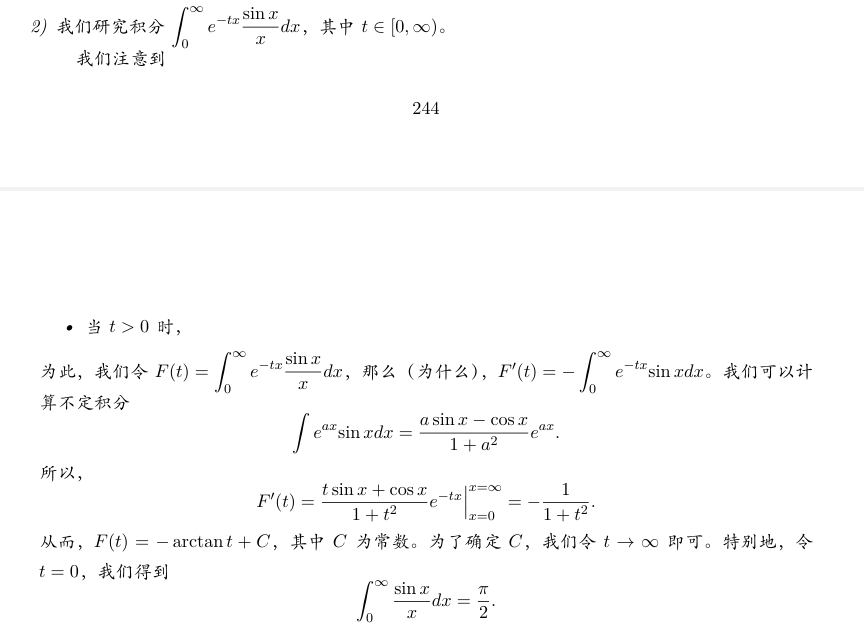
\includegraphics[width=\textwidth]{hw14-2025060817.png}
% \caption{}
\label{}
\end{figure}

首先对于每个 $t>0$,广义积分
\[
\lvert F(t) \rvert \leq \int_{0}^{\infty} \left\lvert  e^{ -tx }\frac{\sin x}{x}  \right\rvert  \, \mathrm{d}x \leq \int_{0}^{\infty} e^{ -tx } \, \mathrm{d}x =\frac{1}{t}<\infty
\]
存在. 且 $f(x,t)=e^{ -tx }\frac{\sin x}{x}$ 关于 $t$ 有偏导数 $f_{t}(x,t)=e^{ -tx }\sin x$,且 $f_{t}$ 在 $[0,\infty)\times[0,\infty)$ 上连续. 接着我们证明 $\int_{0}^{\infty} f_{t}(x,t)\, \mathrm{d}x$,关于 $t>0$ 局部一致收敛,这是因为 $\int_{0}^{N} \sin x \, \mathrm{d}x$ 关于 $t$ 一致有界,且 $e^{ -tx }$ 对于每个给定的 $t$ 都单调递减趋于 0,于是由 Dirichlet 判别法,$\int_{0}^{\infty} f_{t}(x,t) \, \mathrm{d}x$ 关于 $t>0$ 局部一致收敛,因此对于任意 $t>0$,$F'(t)=\int_{0}^{\infty } f_{t}(x,t) \, \mathrm{d}x=-\int_{0}^{\infty} e^{ -tx }\sin x \, \mathrm{d}x$.
